%!TEX TS-program = xetex 
%!TEX encoding = UTF-8 Unicode
\documentclass[letter]{article}

% UTIL

% In case style is not used
\makeatletter
\newcommand{\shorttitle}[1]{}
\newcommand{\authors}[1]{\author{#1}}
\makeatother

\usepackage{ifxetex}

\ifxetex
	\usepackage{polyglossia}
	\setmainlanguage{french}
	\setotherlanguage{latin}
\else
	\usepackage[english, french]{babel}
	\usepackage[utf8]{inputenc}
\fi

\usepackage{float}
\usepackage{array}

\usepackage[top=20mm, bottom=20mm]{geometry}

\usepackage{amsfonts}
\usepackage{amsmath}
\usepackage{amsthm}

\bibliographystyle{alpha}

\usepackage{lipsum}

\usepackage{lscape}
\usepackage{multicol}
\usepackage[french]{minitoc}

\usepackage{ifthen}

\usepackage{datetime}
\usepackage{fancybox}

\usepackage[acronym]{glossaries}
\makeglossary

% Sample 
% \newglossaryentry{sample}{name={sample}, description={A sample entry}}
\newglossaryentry{backface_culling}{name={backface culling}, 
description={(Abattage?) Appelé aussi simplement \eng{culling}, c'est
l'opération consistant à éliminer toutes les faces faisant dos à la caméra et
ne pouvant par conséquent pas être vues.}}

\newglossaryentry{motion_blur}{name={motion blur}, 
description={(Flou de mouvement) C'est le flou généré par une vitesse
d'obturation de la caméra trop grande. }}

\newglossaryentry{clipping}{name={clipping},
description={C'est l'élimination des face hors du champ de la caméra.}}

\newglossaryentry{aliasing}{name={aliasing},
description={Le crénelage sur une image.}}

\newglossaryentry{supersampling}{name={supersampling},
description={Littéralement, sur-échantillonnage, cette technique permet
d'éviter des effets d'aliasing.}}

\newglossaryentry{jittering}{name={jittering},
description={C'est la perturbation que les rayons lumineux subissent
lorsqu'une surface mal polie les réfléchi (par exemple du verre sablé).}}

\newglossaryentry{adaptative_sampling}{name={adaptative sampling},
description={C'est une forme de supersampling qui n'est réalisée que si un
certain seuil d'aliasing est détecté.}}

\newglossaryentry{shader}{name={shader},
description={Un shader est un programme appliqué à l'ensemble des pixel ou des
sommets des polygones de la scène. Ils sont aujourd'hui incorporés dans le
pipeline de rendu des cartes graphiques.}}

% Sample :
% \newacronym{ACA}{ACA}{A Contrived Acronym}
\newacronym{GPU}{GPU}{Graphics Processing Unit}
\newacronym{XP}{XP}{Extrem Programming}



\usepackage{listingsutf8}
\usepackage{xcolor}
\definecolor{colKeys}{rgb}{0,0,1}
\definecolor{colIdentifier}{rgb}{0,0,0}
\definecolor{colComments}{rgb}{0,0.6,0.1}
\definecolor{colString}{rgb}{0.6,0.1,0.1}

\lstset{%configuration de listings 
	float=hbp,% 
		basicstyle=\ttfamily\small, % 
		identifierstyle=\color{colIdentifier}, % 
		keywordstyle=\color{colKeys}, % 
		stringstyle=\color{colString}, % 
		commentstyle=\color{colComments}, % 
		columns=flexible, % 
		tabsize=2, % 
		frame=trBL, % 
		%frameround=tttt, % 
		extendedchars=true, % 
		showspaces=false, % 
		showstringspaces=false, % 
		numbers=left, % 
		numberstyle=\tiny, % 
		stepnumber=2,%
		breaklines=true, % 
		breakautoindent=true, % 
		captionpos=b,% 
		xrightmargin=-1cm, % 
		xleftmargin=-1cm, %
		inputencoding=utf8
}
\lstset{
	literate=	{é}{{\'e}}1
			{è}{{\`e}}1
			{ê}{{\^e}}1
			{à}{{\`a}}1
			{ù}{{\`u}}1
			{ë}{{\"e}}1
			{ô}{{\^o}}1
}


% \code[C++]{Nom du fichier}{Chemin du fichier}
\newcommand{\code}[3][c++]%
{%
	\begin{center}%
		\textbf{#2}%
	\end{center}%
	\lstinputlisting[language=#1]{#3}%
}

\batchmode
\documentclass{article}
\RequirePackage{ifthen}


\usepackage[english, french]{babel}
\usepackage[utf8]{inputenc}


\title{Lyon Ray Tracer}




\usepackage[dvips]{color}


\pagecolor[gray]{.7}

\usepackage[latin1]{inputenc}



\makeatletter

\makeatletter
\count@=\the\catcode`\_ \catcode`\_=8 
\newenvironment{tex2html_wrap}{}{}%
\catcode`\<=12\catcode`\_=\count@
\newcommand{\providedcommand}[1]{\expandafter\providecommand\csname #1\endcsname}%
\newcommand{\renewedcommand}[1]{\expandafter\providecommand\csname #1\endcsname{}%
  \expandafter\renewcommand\csname #1\endcsname}%
\newcommand{\newedenvironment}[1]{\newenvironment{#1}{}{}\renewenvironment{#1}}%
\let\newedcommand\renewedcommand
\let\renewedenvironment\newedenvironment
\makeatother
\let\mathon=$
\let\mathoff=$
\ifx\AtBeginDocument\undefined \newcommand{\AtBeginDocument}[1]{}\fi
\newbox\sizebox
\setlength{\hoffset}{0pt}\setlength{\voffset}{0pt}
\addtolength{\textheight}{\footskip}\setlength{\footskip}{0pt}
\addtolength{\textheight}{\topmargin}\setlength{\topmargin}{0pt}
\addtolength{\textheight}{\headheight}\setlength{\headheight}{0pt}
\addtolength{\textheight}{\headsep}\setlength{\headsep}{0pt}
\setlength{\textwidth}{349pt}
\newwrite\lthtmlwrite
\makeatletter
\let\realnormalsize=\normalsize
\global\topskip=2sp
\def\preveqno{}\let\real@float=\@float \let\realend@float=\end@float
\def\@float{\let\@savefreelist\@freelist\real@float}
\def\liih@math{\ifmmode$\else\bad@math\fi}
\def\end@float{\realend@float\global\let\@freelist\@savefreelist}
\let\real@dbflt=\@dbflt \let\end@dblfloat=\end@float
\let\@largefloatcheck=\relax
\let\if@boxedmulticols=\iftrue
\def\@dbflt{\let\@savefreelist\@freelist\real@dbflt}
\def\adjustnormalsize{\def\normalsize{\mathsurround=0pt \realnormalsize
 \parindent=0pt\abovedisplayskip=0pt\belowdisplayskip=0pt}%
 \def\phantompar{\csname par\endcsname}\normalsize}%
\def\lthtmltypeout#1{{\let\protect\string \immediate\write\lthtmlwrite{#1}}}%
\newcommand\lthtmlhboxmathA{\adjustnormalsize\setbox\sizebox=\hbox\bgroup\kern.05em }%
\newcommand\lthtmlhboxmathB{\adjustnormalsize\setbox\sizebox=\hbox to\hsize\bgroup\hfill }%
\newcommand\lthtmlvboxmathA{\adjustnormalsize\setbox\sizebox=\vbox\bgroup %
 \let\ifinner=\iffalse \let\)\liih@math }%
\newcommand\lthtmlboxmathZ{\@next\next\@currlist{}{\def\next{\voidb@x}}%
 \expandafter\box\next\egroup}%
\newcommand\lthtmlmathtype[1]{\gdef\lthtmlmathenv{#1}}%
\newcommand\lthtmllogmath{\dimen0\ht\sizebox \advance\dimen0\dp\sizebox
  \ifdim\dimen0>.95\vsize
   \lthtmltypeout{%
*** image for \lthtmlmathenv\space is too tall at \the\dimen0, reducing to .95 vsize ***}%
   \ht\sizebox.95\vsize \dp\sizebox\z@ \fi
  \lthtmltypeout{l2hSize %
:\lthtmlmathenv:\the\ht\sizebox::\the\dp\sizebox::\the\wd\sizebox.\preveqno}}%
\newcommand\lthtmlfigureA[1]{\let\@savefreelist\@freelist
       \lthtmlmathtype{#1}\lthtmlvboxmathA}%
\newcommand\lthtmlpictureA{\bgroup\catcode`\_=8 \lthtmlpictureB}%
\newcommand\lthtmlpictureB[1]{\lthtmlmathtype{#1}\egroup
       \let\@savefreelist\@freelist \lthtmlhboxmathB}%
\newcommand\lthtmlpictureZ[1]{\hfill\lthtmlfigureZ}%
\newcommand\lthtmlfigureZ{\lthtmlboxmathZ\lthtmllogmath\copy\sizebox
       \global\let\@freelist\@savefreelist}%
\newcommand\lthtmldisplayA{\bgroup\catcode`\_=8 \lthtmldisplayAi}%
\newcommand\lthtmldisplayAi[1]{\lthtmlmathtype{#1}\egroup\lthtmlvboxmathA}%
\newcommand\lthtmldisplayB[1]{\edef\preveqno{(\theequation)}%
  \lthtmldisplayA{#1}\let\@eqnnum\relax}%
\newcommand\lthtmldisplayZ{\lthtmlboxmathZ\lthtmllogmath\lthtmlsetmath}%
\newcommand\lthtmlinlinemathA{\bgroup\catcode`\_=8 \lthtmlinlinemathB}
\newcommand\lthtmlinlinemathB[1]{\lthtmlmathtype{#1}\egroup\lthtmlhboxmathA
  \vrule height1.5ex width0pt }%
\newcommand\lthtmlinlineA{\bgroup\catcode`\_=8 \lthtmlinlineB}%
\newcommand\lthtmlinlineB[1]{\lthtmlmathtype{#1}\egroup\lthtmlhboxmathA}%
\newcommand\lthtmlinlineZ{\egroup\expandafter\ifdim\dp\sizebox>0pt %
  \expandafter\centerinlinemath\fi\lthtmllogmath\lthtmlsetinline}
\newcommand\lthtmlinlinemathZ{\egroup\expandafter\ifdim\dp\sizebox>0pt %
  \expandafter\centerinlinemath\fi\lthtmllogmath\lthtmlsetmath}
\newcommand\lthtmlindisplaymathZ{\egroup %
  \centerinlinemath\lthtmllogmath\lthtmlsetmath}
\def\lthtmlsetinline{\hbox{\vrule width.1em \vtop{\vbox{%
  \kern.1em\copy\sizebox}\ifdim\dp\sizebox>0pt\kern.1em\else\kern.3pt\fi
  \ifdim\hsize>\wd\sizebox \hrule depth1pt\fi}}}
\def\lthtmlsetmath{\hbox{\vrule width.1em\kern-.05em\vtop{\vbox{%
  \kern.1em\kern0.8 pt\hbox{\hglue.17em\copy\sizebox\hglue0.8 pt}}\kern.3pt%
  \ifdim\dp\sizebox>0pt\kern.1em\fi \kern0.8 pt%
  \ifdim\hsize>\wd\sizebox \hrule depth1pt\fi}}}
\def\centerinlinemath{%
  \dimen1=\ifdim\ht\sizebox<\dp\sizebox \dp\sizebox\else\ht\sizebox\fi
  \advance\dimen1by.5pt \vrule width0pt height\dimen1 depth\dimen1 
 \dp\sizebox=\dimen1\ht\sizebox=\dimen1\relax}

\def\lthtmlcheckvsize{\ifdim\ht\sizebox<\vsize 
  \ifdim\wd\sizebox<\hsize\expandafter\hfill\fi \expandafter\vfill
  \else\expandafter\vss\fi}%
\providecommand{\selectlanguage}[1]{}%
\makeatletter \tracingstats = 1 


\begin{document}
\pagestyle{empty}\thispagestyle{empty}\lthtmltypeout{}%
\lthtmltypeout{latex2htmlLength hsize=\the\hsize}\lthtmltypeout{}%
\lthtmltypeout{latex2htmlLength vsize=\the\vsize}\lthtmltypeout{}%
\lthtmltypeout{latex2htmlLength hoffset=\the\hoffset}\lthtmltypeout{}%
\lthtmltypeout{latex2htmlLength voffset=\the\voffset}\lthtmltypeout{}%
\lthtmltypeout{latex2htmlLength topmargin=\the\topmargin}\lthtmltypeout{}%
\lthtmltypeout{latex2htmlLength topskip=\the\topskip}\lthtmltypeout{}%
\lthtmltypeout{latex2htmlLength headheight=\the\headheight}\lthtmltypeout{}%
\lthtmltypeout{latex2htmlLength headsep=\the\headsep}\lthtmltypeout{}%
\lthtmltypeout{latex2htmlLength parskip=\the\parskip}\lthtmltypeout{}%
\lthtmltypeout{latex2htmlLength oddsidemargin=\the\oddsidemargin}\lthtmltypeout{}%
\makeatletter
\if@twoside\lthtmltypeout{latex2htmlLength evensidemargin=\the\evensidemargin}%
\else\lthtmltypeout{latex2htmlLength evensidemargin=\the\oddsidemargin}\fi%
\lthtmltypeout{}%
\makeatother
\setcounter{page}{1}
\onecolumn

% !!! IMAGES START HERE !!!

{\newpage\clearpage
\lthtmlfigureA{center21}%
\begin{center}\vbox{\section{Auteur}
Je suis Maxime \textsc{Gaudin}, suis élève ingénieur de l'INSA de Lyon en
échange avec l'École Polytechnique de Montréal (attachée à l'Université de
Montréal).

J'étudie en génie informatique et logiciel.

}\end{center}%
\lthtmlfigureZ
\lthtmlcheckvsize\clearpage}

{\newpage\clearpage
\lthtmlfigureA{center22}%
\begin{center}\vbox{\section{Description}
\subsection{Qu'est ce que c'est ?}
\textsl{Lyon Ray Tracer}, en hommage à ma ville natale : Lyon, est un moteur
de rendu utilisant la technique du \textsl{ray tracing} pour produire des
images photoréalistes. Pour ceux qui ne connaissent pas encore le \textsl{ray
tracing}, je vous invite à consulter notre ami \textsl{Wikipedia}
(\url{http://fr.wikipedia.org/wiki/Lancer_de_rayon}).

Par conséquent, mon moteur prend en entrée des informations comme ``il existe
une sphère de centre (0,0,0) et de rayon 10 qui possède un coefficient de
réflexion de 0.5'', et produit le genre d'image de la figure
\ref{fig:spheres}.

\begin{figure}
\begin{center}
  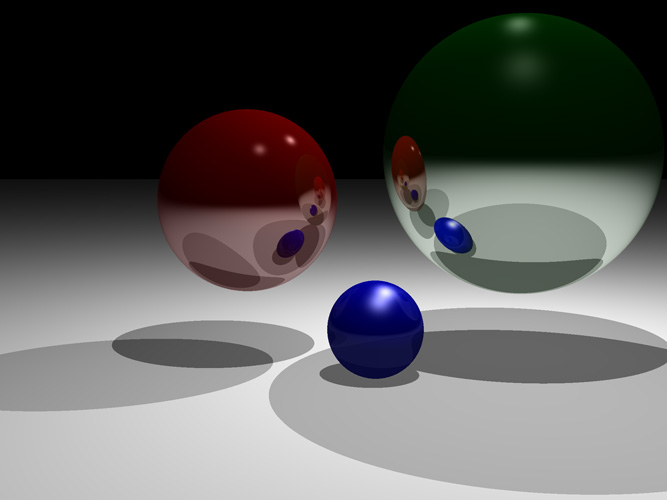
\includegraphics[width=.8\textwidth]{img/spheres}
  \caption{Un exemple de rendu en \textsl{ray tracing}\label{fig:spheres}}
\end{center}
\end{figure}

\subsection{Pourquoi ?}
Bien évidemment parce que j'aime ça ! Mon école ma proposé de réaliser le
projet de mon choix et c'est ce que j'ai choisi. De plus, je trouve que le
concept est formidable : Créer à partir de quelques informations textuelles
des images ultra réalistes et respectant les principes physiques de propagation
de la lumière.

\subsection{Comment ?}
En C++ et en utilisant le plus d'outils libres et standards. Pour vous donner
une idée de mon toolkit, je vous conseil d'aller jeter un coup d'œil du côté
des dépendances.

\subsection{C'est cool, je peux participer ??}
Oh oui !\\

Un moteur de \textsl{ray tracing} c'est comme des Légo, on peu toujours
ajouter quelques choses (surtout en ce moment, puisque le moteur n'est pas
encore très évolué). C'est donc pour toi l'occasion de participer à quelques
choses au tout début de son évolution.\\

Tu peux par exemple :
\begin{itemize}
  \item Me laisser un petit mail pour m'encourager !
  \item Essayer de compiler le programme et m'avertir des différents problèmes
    que tu as pu rencontrer (si possible avec la solution ;) )
  \item M'envoyer des \textsl{pull requests} (même si c'est pour un coquille
    ou ajouter un peu de documentation).
  \item M'aider à créer une vraie page web au lieux de ce PDF :p
\end{itemize}

\subsection{Fonctionnalités}
\paragraph{Lumières}
\begin{itemize}
  \item Lumière directionnelle.
\end{itemize}

\paragraph{Caméra}
\begin{itemize}
  \item Caméra classique avec prise en compte de la perspective.
\end{itemize}

\paragraph{Géométrie}
\begin{itemize}
  \item Sphère.
  \item Plan infini.
\end{itemize}

\paragraph{Matériaux}
\begin{itemize}
  \item Couleur diffuse, spéculaire, ambiante.
  \item Indice de réfraction.
  \item Indice de réflexion.
\end{itemize}

\paragraph{Importeurs}
\begin{itemize}
  \item 3DS.
\end{itemize}

\paragraph{Exporteurs}
\begin{itemize}
  \item PNG.
  \item JPG.
\end{itemize}

}\end{center}%
\lthtmlfigureZ
\lthtmlcheckvsize\clearpage}

{\newpage\clearpage
\lthtmlfigureA{center23}%
\begin{center}\vbox{\section{Dépendences}
La compilation du projet nécessite :
\begin{enumerate}
  \item Un compilateur C++ récent (\textsl{i.e.} gcc 4.2+)
  \item make
  \item boost
  \item libjpeg
  \item libpng
\end{enumerate}

}\end{center}%
\lthtmlfigureZ
\lthtmlcheckvsize\clearpage}

{\newpage\clearpage
\lthtmlfigureA{center24}%
\begin{center}\vbox{\section{Licences}
À priori, LGPL.

}\end{center}%
\lthtmlfigureZ
\lthtmlcheckvsize\clearpage}


\end{document}

\newcommand{\ie}{\textsl{i.e.}~}
\newcommand{\cf}{\textsl{Cf.}~}
\newcommand{\etc}{\textsl{etc.} }
\newcommand{\eg}{\textsl{e.g.}~}

\newcommand{\apriori}{\textsl{a priori}~}
\newcommand{\Apriori}{\textsl{A priori}~}

\newcommand{\resp}{\textsl{resp.}~}

\newcommand{\nb}[1]{\vspace*{\fill}\sl{\sc Nota bene} : #1}

\newcommand{\wrt}{\textsl{w.r.t.~}}
\newcommand{\Wrt}{\textsl{W.r.t.~}}

% This file is a part of ShaperPerfect Article 2.0
% and entirely the property of Maxime Gaudin.
%
% 2011

\newcommand{\tsl}[1]{\textsl{#1}}
\newcommand{\tbf}[1]{\textbf{#1}}
\newcommand{\ttt}[1]{\texttt{#1}}
\newcommand{\tsc}[1]{\textsc{#1}}

\newcommand{\ie}{\textsl{i.e.}\ }
\newcommand{\cf}{\textsl{Cf.}\ }
\newcommand{\etc}{\textsl{etc.}}
\newcommand{\eg}{\textsl{e.g.}\ }

\newcommand{\resp}{\textsl{resp.}\ }

\newcommand{\wrt}{\textsl{w.r.t.}\ }
\newcommand{\Wrt}{\textsl{W.r.t.}\ }

\newcommand{\gfont}{%
	\fontencoding{\encodingdefault}%
	\fontfamily{ptm}%
	\fontseries{bc}%
	\fontshape{bf}%
	\fontsize{65}{60}%
	\selectfont}

% \quote[Auteur]{Citation}
\renewcommand{\quote}[2][null]
{%
	~\\
	\begin{minipage}{\textwidth}%
	\vspace*{\baselineskip}
		\parbox{0.2\textwidth} {\textcolor[rgb]{0.5,0.5,0.5}{\gfont "}}%
			\parbox{0.8\textwidth}%
			{%
				\textcolor[rgb]{0.3, 0.3, 0.3}{\textsl{#2}}%
				\ifthenelse{\equal{#1}{null}}{}{\begin{flushright}\textsc{#1}\end{flushright}}%
			}%
	\end{minipage}%
}%

\newlength{\parindentCopy}
\setlength{\parindentCopy}{\parindent}

%%% Indentation correction
\newcommand{\newpar}[0]
{
	~\\
	\hspace*{0.8\parindent}
}
%
\newenvironment{unindent}
{
	\setlength{\parindent}{0pt}
}
{
	\setlength{\parindent}{\parindentCopy}
}

\newcommand{\checked}[1]
{%
	\begin{center}%
	        \textcolor[rgb]{0.0, 0.9, 0.2}{\large\checkmark}#1%
	\end{center}%
}

\usepackage{hyperref}
\hypersetup{
	backref=true,                           % Permet d'ajouter des liens dans
	pagebackref=true,                       % les bibliographies
	hyperindex=true,                        % Ajoute des liens dans les index.
	colorlinks=true,                        % Colorise les liens.
	breaklinks=true,                        % Permet le retour à la ligne dans les liens trop longs.
	urlcolor= blue!80,                         % Couleur des hyperliens.
	linkcolor= black!60,                        % Couleur des liens internes.
	bookmarks=true,                         % Créé des signets pour Acrobat.
	bookmarksopen=true,                     % Si les signets Acrobat sont créés,
}

\ifxetex
	\usepackage{xunicode}
	\usepackage{xltxtra}
	\usepackage{fontspec}
	
	\defaultfontfeatures{Mapping=tex-text}
	
	\newcommand{\tmpfont}[3][null]
	{%
		\ifthenelse{\equal{null}{#1}}%
		{{\fontspec{#2}#3}}%
		{{\fontspec[#1]{#2}#3}}%
	}%

	\newcommand{\og}{«}
	\newcommand{\fg}{»}
\fi

\usepackage{type1cm}
\usepackage{eso-pic}
\usepackage{color}

\makeatletter
\def\draft{ 
	\AddToShipoutPicture{%
		\setlength{\@tempdimb}{.5\paperwidth}%
			\setlength{\@tempdimc}{.5\paperheight}%
			\setlength{\unitlength}{1pt}%
			\put(\strip@pt\@tempdimb,\strip@pt\@tempdimc){%
				\makebox(0,0){\rotatebox{45}{\textcolor[gray]{0.95}%
					{\fontsize{6cm}{6cm}\selectfont{DRAFT}}}}%
			}%  
	}   
}
\makeatother


\newenvironment{deprecated}
{%
	\color{gray}%
	\textsc{Deprecated}\hrulefill
}
{%
\hrule%~\\
}

\newcommand{\pref}[1]{[\tsl{p.\ref{#1}}]}
\newcommand{\fref}[1]{\tsl{fig.} \ref{#1}}
\newcommand{\Fref}[1]{\tsl{Fig.} \ref{#1}}


\usepackage{fancyhdr}
\pagestyle{fancy}

\fancyhf{}
\renewcommand{\headrulewidth}{0pt}

\makeatletter
\fancyfoot[C]{\bf\sp@shorttitle}
\makeatother

% Heading des pages de style plain
\fancypagestyle{plain}{%
	\fancyhf{}%
	\renewcommand{\headrulewidth}{0pt}%
}

\newdateformat{veryshortdate}{\monthname[\THEMONTH] \THEYEAR}

\newcommand{\titlefont}{%
\fontencoding{\encodingdefault}%
\fontfamily{pag}%
\fontseries{bc}%
\fontshape{n}%
\fontsize{25}{20}%
\selectfont}%

\newcommand{\authorsfont}{%
\fontencoding{\encodingdefault}%
\fontfamily{pag}%
\fontseries{bc}%
\fontshape{n}%
\fontsize{8}{5}%
\selectfont}%

\newlength{\titlehruleheight}
\setlength{\titlehruleheight}{0.3mm}

\makeatletter
%Default values
\def\sp@title{Titre}
\def\sp@shorttitle{}
\def\sp@authors{Auteurs}

\renewcommand{\title}[1]{\def\sp@title{#1}}
\renewcommand{\shorttitle}[1]{\def\sp@shorttitle{#1}}
\renewcommand{\authors}[1]{\def\sp@authors{#1}}
%\newcommand{\logo}[1]{\def\sp@logo{#1}}

\renewcommand{\maketitle}
{%
	\thispagestyle{fancy}%
	\begin{center}\titlefont\sp@title\\\end{center}%
	{\authorsfont\sl\sp@authors\hfill\veryshortdate\today}~\\%
	\hrule height \titlehruleheight%
	\vspace*{0.5cm}%
}
\makeatother

%\input{../build/shapeperfect/style/customPart}
\newlength{\sectiontitleindent}
\setlength{\sectiontitleindent}{-1cm}

\newlength{\subsectiontitleindent}
\setlength{\subsectiontitleindent}{-.5cm}

\newlength{\subsubsectiontitleindent}
\setlength{\subsubsectiontitleindent}{-.25cm}

\newlength{\paragraphtitleindent}
\setlength{\paragraphtitleindent}{-.125cm}

\newcommand{\sectionfont}{
	\fontencoding{\encodingdefault}
	\fontfamily{pag}
	\fontseries{bc}
	\fontshape{n}
	\selectfont}

\makeatletter
\renewcommand{\section}{
	\@startsection
	{section}
	{1}
	{\sectiontitleindent}
	{-3.5ex plus -1ex minus -.2ex}
	{2.3ex plus.2ex}
	{\sectionfont\Large}}

\renewcommand{\subsection}{
 	\@startsection
 	{subsection}
 	{2}
 	{\subsectiontitleindent}
 	{-3.5ex plus -1ex minus -.2ex}
 	{2.3ex plus.2ex}
 	{\sectionfont\large}}

\renewcommand{\subsubsection}{
 	\@startsection
 	{subsubsection}
 	{3}
 	{\subsubsectiontitleindent}
 	{-3.5ex plus -1ex minus -.2ex}
 	{2.3ex plus.2ex}
 	{\sectionfont}}

\renewcommand{\paragraph}{
 	\@startsection
 	{paragraph}
 	{4}
 	{\paragraphtitleindent}
 	{-3.5ex plus -1ex minus -.2ex}
 	{2.3ex plus.2ex}
 	{\sectionfont\normalsize\bf}}
\makeatother

\fancyheadoffset[LO]{33mm}
\fancyheadoffset[R]{32mm}
%\fancyhead[LE]{\rightmark}
%\fancyhead[RO]{\leftmark}
\renewcommand{\headrulewidth}{0pt}

\fancyhead[L]
{
	\ifthenelse{\isodd{\thepage}}{}{%
		\rotatebox{-90}{%
			\hbox to 0pt{%
				\Huge\fontfamily{ugq}\selectfont\rotatebox{180}{\fboxsep=20pt\colorbox{white}{\color{gray}\thepage}}\hbox to 0.3cm{}%
			}%
		}%
		\vspace*{-100mm}
	}%
}

\fancyhead[R]
{
	\ifthenelse{\isodd{\thepage}}{%
		\raisebox{0pt}[0pt][0pt]{
		\raisebox{-16.6cm}{%
			\rotatebox{90}{%
				\hbox to 0pt{%
					\Huge\fontfamily{ugq}\selectfont\rotatebox{180}{\fboxsep=20pt\colorbox{white}{\color{gray}\thepage}}\hbox to 0.3cm{}%
				}%
			}%
		}%
		}%
	}{}%
}

\addto\captionsfrench{\renewcommand*{\glossaryname}{Glossaire}}
\addto\captionsfrench{\renewcommand*{\acronymname}{Liste des accronymes}}

\newcommand{\gBox}[1]{% 
	\shadowbox{\sffamily#1}\\\hfill\mbox{}%
}

\newglossarystyle{nation}{%
	\renewenvironment{theglossary}{\begin{description}}{\end{description}}%
	\renewcommand*{\glossaryheader}{}%
	\renewcommand*{\glsgroupheading}[1]{}%
	\renewcommand*{\glsgroupskip}{}%
	\renewcommand*{\glossaryentryfield}[5]{%
	\item % bullet point
	\gBox{\glstarget{##1}{\uppercase{##2}}}% the entry name
	\space {##3}% the description
	\space [Page(s) ##5]\\% the number list in square brackets
	}%
	\renewcommand*{\glossarysubentryfield}[6]{%
		\glossaryentryfield{##2}{##3}{##4}{##5}{##6}}%
}
\glossarystyle{nation}


\usepackage{float}
\usepackage{tikz}
\usetikzlibrary{shapes.multipart} 

\newcommand{\eng}[1]{\tsl{#1}}

\newcommand{\raytracing}[0]{\eng{raytracing}}
\newcommand{\remark}[1]{

\vspace*{1em}\hspace*{\fill}\begin{minipage}{.8\textwidth}
\it\tbf{Remarque :} #1
\end{minipage}
}
\safeusepackage{wasysym}

\newcommand{\gfont}{%
	\fontencoding{\encodingdefault}%
	\fontfamily{ptm}%
	\fontseries{bc}%
	\fontshape{bf}%
	\fontsize{65}{60}%
	\selectfont}

% \quote[Auteur]{Citation}
\renewcommand{\quote}[2][null]
{%
	~\\
	\begin{minipage}{\textwidth}%
	\vspace*{\baselineskip}
		\parbox{0.2\textwidth} {\textcolor[rgb]{0.5,0.5,0.5}{\gfont "}}%
			\parbox{0.8\textwidth}%
			{%
				\textcolor[rgb]{0.3, 0.3, 0.3}{\textsl{#2}}%
				\ifthenelse{\equal{#1}{null}}{}{\begin{flushright}\textsc{#1}\end{flushright}}%
			}%
	\end{minipage}%
}

\usepackage{subfigure}
\usepackage{wrapfig}

\usepackage{titlesec}
\titlespacing{\paragraph}
{0pt}
{0.5\baselineskip}
{.35em}


\title{INF4000 : Projet personnel}
\authors{Maxime \tsc{Gaudin}}
\shorttitle{}

\newcommand{\raytracing}[0]
{\tsl{ray tracing} }

\begin{document}
\maketitle

Le \raytracing est une technique de synthèse d'image consistant à simuler le
parcours de la lumière mais en chemin inverse. En effet, puisqu'il serait bien
trop complexe de suivre la lumière de la source (\eg d'une lampe de poche)
jusqu'à l'objectif, et ce, en calculant toutes les interactions possibles avec
l'environnement, l'algorithme effectue le chemin inverse : De l'objectif à
l'environnement. 

\newpar Cette technique est utilisée dans de nombreux domaines allant de
l'imagerie médicale, en passant par la représentation 3D de systèmes complexes
jusqu'au cinéma.

\newpar Enfin, afin de rendre le sujet encore plus interessant, j'aimerais
tenter d'implémenter la technique de cartographie de photons, permettant de
simuler des interactions lumineuses telles que les caustiques.

\section{Spécification du projet}
\subsection{Liste des fonctionnalités}
\begin{enumerate}
  \item Un moteur de \raytracing ``classique''. \tick
  \item La gestion de primitives (sphères, plan, tores, et en général toutes
    les figures ayant une représentation paramétrique).
  \item La gestion de plusieurs types de caméras : Orthographique,
    perspective, \etc
  \item La gestion de plusieurs types de lumières : Point, plan, sphérique,
    \etc.
  \item La gestion d'au moins un format de représentation polygonale.
  \item La mise en place des structures accélératrices.
\end{enumerate}

Comme spécifié plus haut, il serait intéressant d'implémenter la cartographie
des photons mais j'ai peur que le nombre d'heures allouées au projets ne
me permettent pas de le faire.

\subsection{Aspects de conception}
La technique du \raytracing, bien que très simple, nécessite une architecture
logicielle très bien conçu car le développement de ce genre de programme se
faire de manière incrémentale et itérative (d'autant plus lorsqu'il n'y a
qu'un seul développeur). 

\end{document}

